\section{Visualisierung der Daten anhand eines Netzwerkes}\label{network}

Während Sequential Pattern Mining lediglich häufige Sequenzen in den Daten findet, sollen die Daten zusätzlich noch in Form eines Netzwerkes dargestellt werden. Dies ermöglicht die Visualisierung des kompletten Datensatzes und liefert weitere Informationen bezüglich von Mustern in den Daten.\\
Zum bessern Verständnis sollen an dieser Stelle einige elementare Grundlagen der Graphentheorie vorgestellt werden. Ein geordneter Graph $G=(V,E)$ besteht aus einer Menge $V$ von Knoten und einer Menge $E$ von Kanten. Eine Kante $e_i \in E$ besteht aus einem geordneten Paar von zwei Knoten $(v_j,v_k)$, wobei $v_j,v_k \in V$. Das heißt eine Kante stellt die geordnete Verbindung zwischen zwei Knoten dar \cite[16]{network_data}.\\
Das Netzwerk ist wie folgt strukturiert. Ausgehend von einem Startpunkt führen $17$ Kanten zu den $17$ Kampagnen der ersten Position. Diese $17$ Kampagnen entsprechen jeweils einem Knoten. Die Namen der Knoten setzen sich aus dem Namen der Kampagne und $\_1$ für Position $1$ zusammen. Von jeder Kampagne führt dann eine Kante zu $Success\_1$ für die Funnels, die nach einem Kontakt konvertiert sind sowie eine Kante zu $Fail\_1$ für die Funnels, deren Beobachtung nach einem Konaktpunkt ohne Konvertierung abbricht. Außerdem führen von jeder der $17$ Kampagnen der ersten Position jeweils $17$ Kanten zu den $17$ Kampagnen der zweiten Position. Die Knoten der zweiten Position setzen sich wiederum aus dem Namen der Kampagne und $\_2$ zusammen. Von dort führen wieder Kanten zu $Success\_2$, $Fail\_2$ und den Kampagnen der dritten Position. Dieses Prinzip setzt sich für die weiteren Positionen fort.\\
Diese Kanten werden bezüglich der Anzahl der Nutzer gewichtet. Anhand imaginärer Zahlen soll hier das Prinzip kurz dargestellt werden. Wenn $50000$ Nutzer als ersten Kontakt $Direct$ haben, so hat der Knoten $Direct\_1$ ein Gewicht von $50000$. Diese verteilen sich nun auf die Knoten, die mit $Direct\_1$ durch eine Kante verbunden sind. Wenn die Kante zwischen $Direct\_1$ und $Direct\_2$ beispielsweise ein Gewicht von $10000$ hat, so haben $10000$ Nutzer als ersten und zweiten Kontakt $Direct$. Wenn die Kante zwischen $Direct\_1$ und $Success\_1$ ein Gewicht von $500$ hat, so bedeutet das, dass $500$ Nutzer als ersten Kontakt $Direct$ haben und danach direkt konvertieren.\\
Um aussagekräftigere Ergebnisse zu erzielen, wurden für die Gewichtung der Kanten nicht die absoluten Anzahlen gewählt. Stattdessen wurden zwei Strategien verfolgt, die im folgenden als relative Ausgänge beziehungsweise relative Eingänge bezeichnet werden. Für die relativen Ausgänge werden die Kanten mit den relativen Häufigkeiten gewichtet, wobei die zugrundeliegende Menge die Summe aller Nutzer ist, die einen Knoten verlassen. Das heißt die Summe der Gewichte aller Kanten, die einen Knoten verlassen ergeben in der Summe $1$. Wenn nun das Gewicht der Kante zwischen $Direct\_2$ und $Fail\_2$ $0.2$ entspricht, so sind $20 \%$ der Nutzer, die als zweiten Kontakt $Direct$ haben, nach dem zweiten Kontaktpunkt konvertiert. Diese Gewichtung erlaubt somit eine relative Betrachtung der Kanten die eine Kampagne verlassen.\\
Für die relativen Eingänge werden die Kanten ebenfalls mit den relativen Häufigkeiten gewichtet, wobei die zugrundeliegende Menge nun die Summe aller Nutzer ist, die in einen Knoten gehen. Betrachtet man beispielsweise $Success\_2$, so kann man erkennen, aus welchen Kampagnen der zweiten Position sich die konvertierten Funnels der Länge $2$ zusammen setzen. Hat die Kante zwischen $Direct\_2$ und $Success\_2$ nun einen Gewicht von $0.2$, so haben $20 \%$ der konvertierten Funnels der Länge $2$ als letzten Kontaktpunkt vor der Konvertiertung $Direct$. Somit sind zwei verschiedene Interpretationsmöglichkeiten durch die unterschiedliche Gewichtung der Kanten gegeben.\\
Das Netzwerk mit den gewichteten Kanten wird in \textit{R} mit dem Paket \textit{rgexf} \cite{rgexf} erzeugt und als \textit{gexf}-Datei exportiert. Daraufhin wird die Datei in das Open-Source Programm \textit{Gephi} \cite{gephi_bastian} geladen. Dort werden die Daten dann als Graph dargestellt. Abbildung \ref{graphbegin} zeigt die räumliche Anordnung der Knoten und Kanten nach dem ersten Einlesen der \textit{gexf}-Datei in \textit{Gephi}, die noch willkürlich ist. Die farbigen Punkte sind die Knoten und die Linien die Kanten.\\
Für die Berechnung der räumlichen Anordnung der Knoten und Kanten stehen in \textit{Gephi} einige Algorithmen zur Verfügung. Diese berechnen die Anordung der Knoten anhand der Anziehungs- beziehungsweise Abstoßungskraft der Knoten, die aus den relativen Häufigkeiten resultieren. Stärker verbundene Knoten liegen damit näher beieinander als schwach verbundene. Das heißt Knoten, die überhaupt keine Verbindung enthalten, liegen weiter auseinander. Ein Beispiel wäre $Direct\_1$ und $Direct\_3$, da man von der ersten Position nicht direkt zur dritten Position springen kann, sondern zunächst einen Kontaktpunkt an der zweiten Position benötigt. Durch die Anwendung eines Algorithmus ergibt sich somit eine lineare Struktur, die die Positionen aneinander reiht.\\
Für diese Arbeit wurden der Algorithmus \textit{Force Atlas 2} \cite{forceatlas2} und der Algorithmus nach \textit{Yifan Hu} \cite{yifanhu} verwendet, wobei \textit{Yifan Hu} das Netzwerk besser in einzelne Ebenen einteilen kann. Das heißt die Positionen sind hier räumlich deutlicher getrennt. Für die Präsentation der Ergebnisse in Kapitel \ref{resultsnetwork} wurde die räumliche Anordnung der Knoten allerdings noch manuell bearbeitet, um die Ergebnisse anschaulicher zu machen.\\
\begin{figure}[H]
	\centering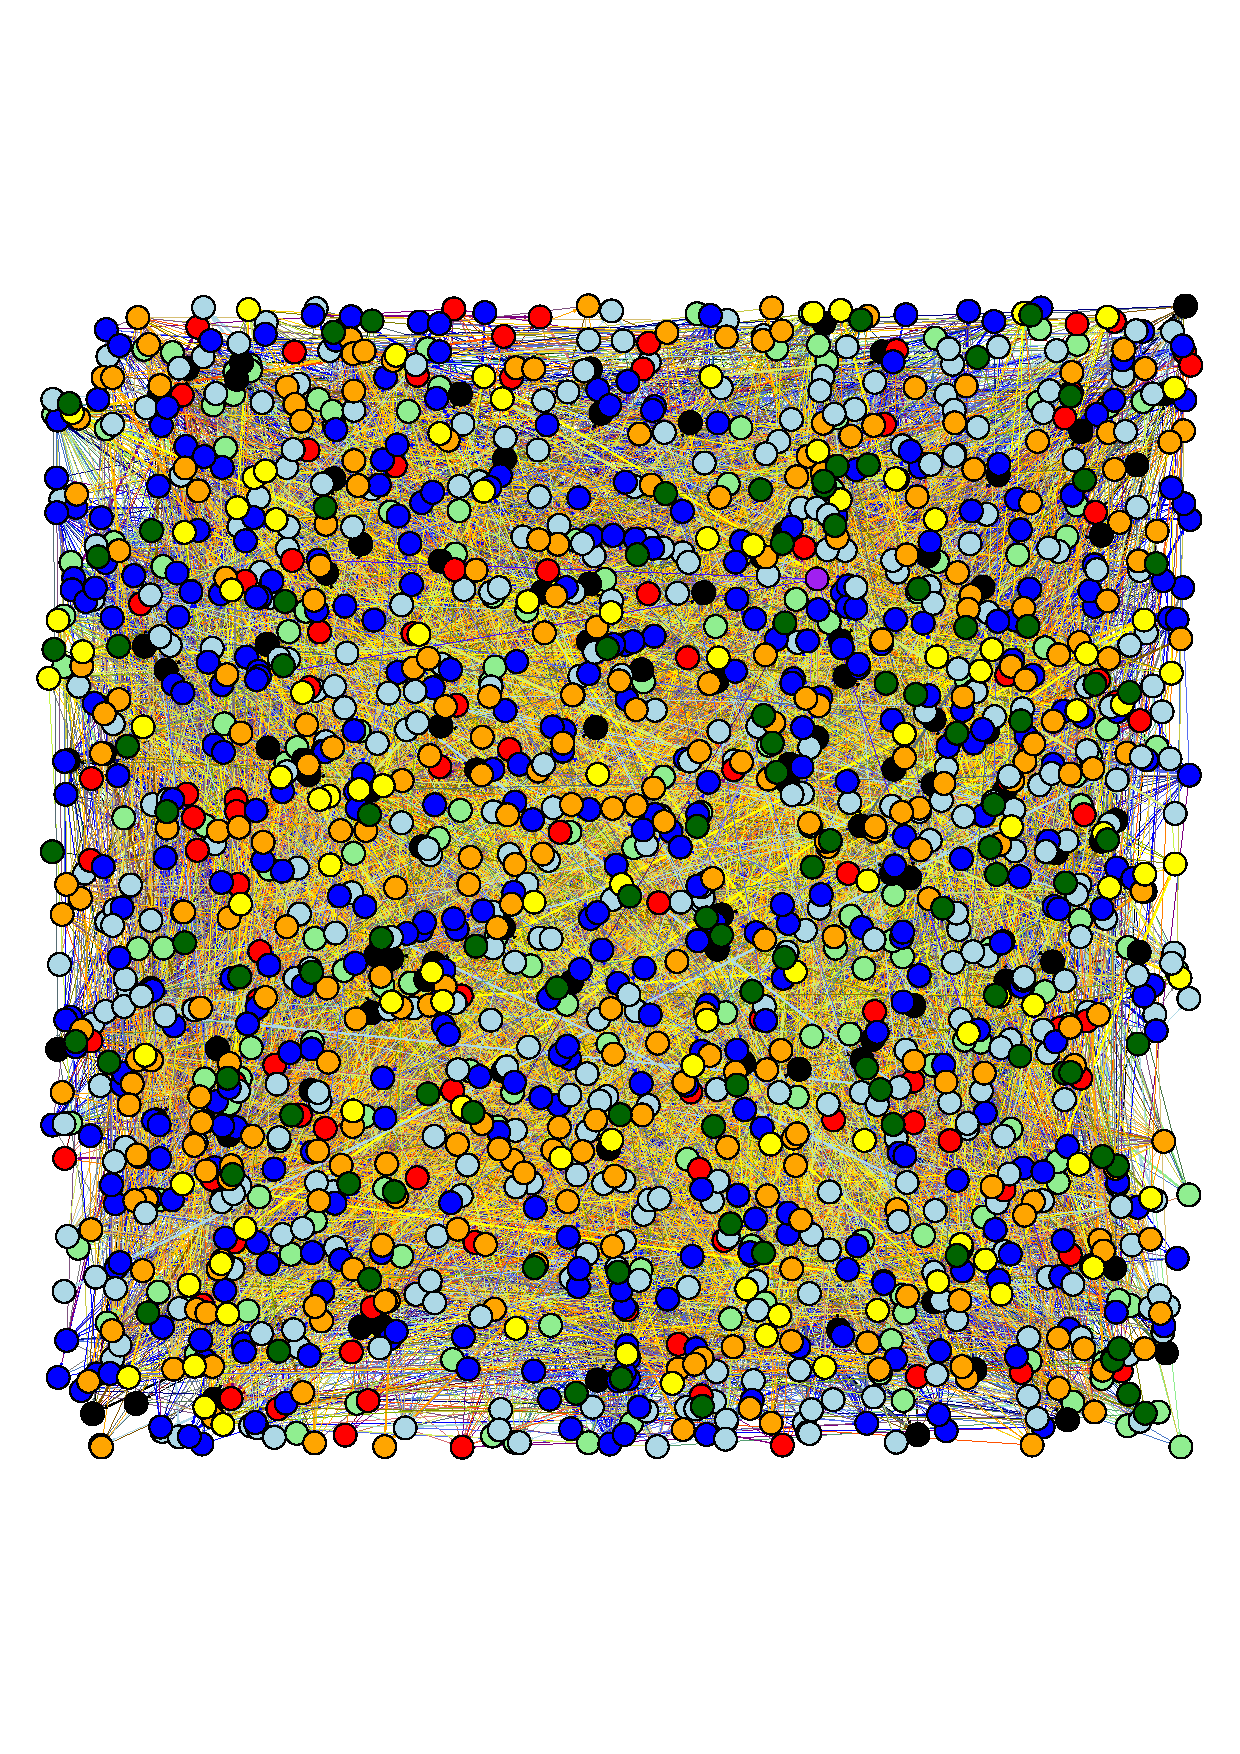
\includegraphics[scale=0.5]{graphbegin.pdf}\caption[Anordnung der Knoten nach dem Einlesen]{Anordnung der Knoten und Kanten direkt nach dem Einlesen in Gephi}\label{graphbegin}
\end{figure}
\noindent Das Netzwerk kann in \textit{Gephi} interaktiv bearbeitet werden. Die Daten sowie das Programm sind im elektronischen Anhang enthalten und werden in Kapitel \ref{anhang} näher beschrieben.



